%=========================================================================
% (c) Michal Bidlo, Bohuslav K�ena, 2008

\chapter{FreeIPA}

FreeIPA (where IPA stands for Identity, Policy and Audit) is an open-source security management solution sponsored by Red Hat aimed primarily at Linux and Unix machines\cite{ipaWeb}.

The project itself combines a number of various existing open-source technologies to achieve the goal of providing centralized authentication and authorization, as well as storing important account information like users or group memberships.
FreeIPA also aims to provide easy management and setup of a domain controller which would otherwise be very difficult by using the same components on your own.

In this chapter I will briefly introduce some of the components FreeIPA uses and describe the architecture of the resulting FreeIPA server solution.

\section{Directory Server}
FreeIPA's directory service is the foundation of the whole solution as it stores various information on behalf of all of FreeIPA's components.
It also plays a big role in authentication and authorization using Kerberos which will be presented in the next section.

The LDAP protocol\cite{ldapRFC} is used as a means of communication with the server and the data itself is stored in a Directory Information Tree (DIT) which is a tree-like data structure.

LDAP provides several operations to use with the server\cite{ldapRFC}:

\begin{itemize}
    \item \textbf{add, delete, modify:} These operations add, remove and modify the data contained in the DIT.
    \item \textbf{search, compare:} The search and compare operations are used in querying the DIT for specific information.
    \item \textbf{bind, unbind, abandon:} These operations can be used to authenticate to the directory, terminating the connection or abandoning a previously sent request entirely, respectively.
    \item \textbf{extended operations:} New operations that are not a part of the original protocol.
\end{itemize}

The actual LDAP compatible server is implemented using the 389 Directory Server project\cite{ldapWeb}.
% TODO: ACLs

\section{Kerberos}
Kerberos\cite{kerbRFC} is a network authentication protocol that uses symmetric encryption using a pre-shared key to authenticate the client to a network service (and vice versa) via an insecure connection using a trusted third party service called a Key Distribution Center (KDC). \\
The resulting communication is secure because no secret keys are transported over the network in plaintext format as the KDC already contains a database of credentials for users and services in the Kerberos realm. \\

\begin{figure}[!ht]
    \centering
        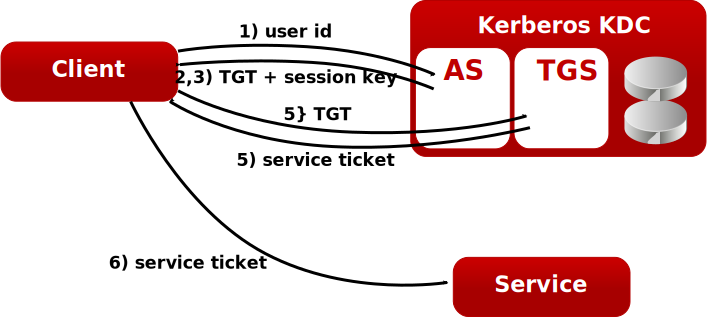
\includegraphics[scale=0.6]{fig/kerb}
    \caption{Kerberos authentication process.}
    \label{fig:kerb}
\end{figure}

The process of authenticating the user to a network service is shown in figure \ref{fig:kerb} and can be described in these steps:
\begin{enumerate}
    \item The user sends his principal name (an unique identifier) to the KDC's Authentication Server (AS) via a plaintext request.
    \item The AS then checks the database to make sure the user exists and sends back a randomly generated session key to be used to encrypt communication with another service called a Ticket-Granting Service (TGS) encrypted with the user's secret key.
    \item The AS also generates a set of credentials called a Ticket-Granting Ticket (TGT) which includes the previously generated session key and is encrypted by the secret key of the TGS.
    \item After recieving the first message the client decrypts it using his secret key. This is the only time the user's key is actually used. The TGT which the client can't decrypt himself is saved in a cache on the client's side to be used later to setup a session with the TGS. At this point the user is authenticated to the Kerberos realm and doesn't have to input his secret key again for a set amount of time (commonly 10-24 hours).
    \item When the user wants to authenticate agains a service in the Kerberos realm he just has to ask the TGS to send him a ticket.
    \item The user then authenticates to the chosen service using this ticket without the need for his secret key.
\end{enumerate}

As the security of the Kerberos protocol is partly based on the time stamps of tickets, all of the clients and services in the realm have to be properly synchronized time-wise. To achieve this goal the Network Time Protocol is used in the FreeIPA project. \\
FreeIPA's KDC is implemented using the MIT Kerberos\cite{kerbWeb} open source software and FreeIPA also provides its own KDC data backend called ipa-kdb which is used to both read and write user information to FreeIPA's LDAP directory service\cite{kerbIpa}.
\section{DNS}
Even though it would be possible to access network services located in a FreeIPA domain directly using their IP addresses, it is much more easier to do so using domain names. \\
The Domain Name System (DNS)\cite{dnsRFC} is distributed naming system, that translates domain names, which can be easily memorized by humans, into IP addresses using special name servers.
As such if one wants to access a network service or a webpage he doesn't have to remember its IP address, only the IP address of the name server (which is stored localy on the client machine) and the domain name of the service/webpage. \\
The domain name space resembles a tree structure, each node having a label that designates a part of its domain name, while the full domain name of the node can be built by concatenating this label with the domain name of its parent node. \\
The name space is divided into zones starting at the root of the tree structure with child nodes of the root node called top-level domains (TLD).
These zones can contain one or several domains, each domain served by one or several name servers, and can be divided into additional zones if deemed necessary. \\
The DNS server in FreeIPA uses a enhanced BIND name server which allows FreeIPA to store data into a LDAP directory\cite{dnsIpa}.
However using FreeIPA's integrated DNS server is optional and as such the project can be used with a different third party DNS server if so desired.
\section{FreeIPA Architecture}
\begin{figure}[!ht]
    \centering
        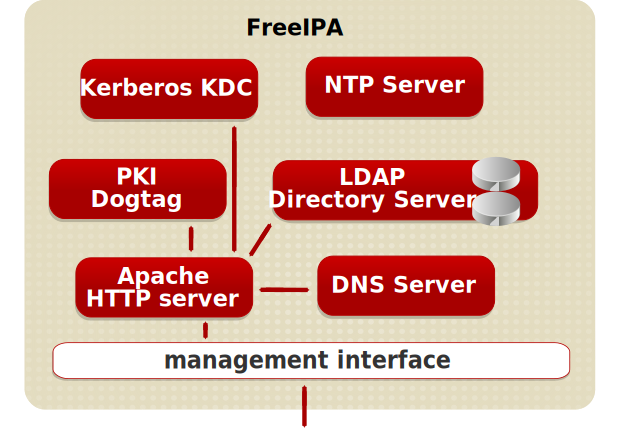
\includegraphics[scale=0.6]{fig/ipa-architecture}
    \caption{FreeIPA server architecture.}
\end{figure}

\section{Extending FreeIPA}
\subsection{Extending the Framework}
\subsection{Extending the Directory Server}

\chapter{Active Directory}
\chapter{Analyze}
\chapter{Conclusion}

%=========================================================================
